\section{Introduction}

An assistant is useful partly because we do not have to tell it everything
again. It can remember a preference, a plan, or something we mentioned weeks
ago. But keeping that information should also be a choice. A patient detail
entered in the wrong conversation should be removable without losing the
rest of the case, just as an incident-response assistant should let us remove
a temporary access token while keeping the troubleshooting history. We study
this selective request through a simpler conversation about bicycles and
travel, adapted from separate public LongMemEval exchanges~\citep{longmemeval}:

\begin{quote}
\textbf{Keep the earlier exchange:} The user describes a road bike, a
mountain bike, and a commuter bike.\\
\textbf{Delete the later exchange:} The user reports buying a hybrid and
now having four bikes. The assistant congratulates the user and repeats
the four-bike total.\\
\textbf{Keep the unrelated exchange:} The assistant supplies contact
details for the Speyer tourism board.
\end{quote}
The user now asks: ``Please forget the update where I said I now
own four bikes. Keep the rest of our conversation, including the Speyer
contact details.'' We add this request to the benchmark and remove the
user's update together with the assistant's reply, because the reply repeats
the information. The earlier three-bike discussion remains. We have two
questions to ask afterward: how many bikes does the user own, and what was
that tourism board's phone number? This case measures the model's
probabilities for the saved answers (Appendix~\ref{app:bicycle-case}); we
also test generated answers in a separate mortgage case
(Section~\ref{sec:mortgage-case}).

The conversation we can read and the memory the model has computed from it
are different objects. GemmaSV edits the latter: the stored key and value
vectors used to produce a reply. We install a support-vector gate in the
global attention layers of frozen Gemma~3 and record which memory rows each
exchange owns. A deletion request can then locate those rows and exclude
them from the readout; we call this an \emph{addressable} memory. The
pretrained parameters stay unchanged, without adapter, distillation, or
recovery training. The visible transcript and any copies in external logs or
databases require separate handling.

Suppose the assistant answers that it does not remember the bicycle update.
Did the information go away, or did the assistant just avoid saying it? We
need to check both the answers and the memory change. For the memory, an
independent \emph{local refit} recalculates the gate on the surviving stored
rows, allowing us to check whether the requested edit was carried out.
However, later rows may already have been influenced by the exchange when
they were encoded. We therefore also run the model again on the conversation
with that exchange omitted. This \emph{raw-history rebuild} recomputes the
surviving rows as well as the gate. Comparing the edit with both references
lets us examine how much of the original exchange's influence remains after
its own rows have been excluded.

We use the support-vector gate of~\citet{svattn} and the decremental learning
method of~\citet{cp2000} to test whether this interface can be added to a
released model without further training. The experiments identified a 4B
configuration with a modest paired perplexity cost on the tested text; the
same configuration lost admission at 1B and 12B. At the selected scale, the
model disclosed fewer deleted answers than under a prompt instruction to
forget. Yet an attack could still detect that some records had been stored,
and the long-history probability tests separated editing from rebuilding.

\section{Related Work}\label{sec:related}

Unlearning methods such as negative preference
optimization~\citep{zhang2024npo} modify pretrained parameters. TOFU, MUSE,
and WMDP evaluate how these changes affect forgotten and retained
information~\citep{tofu,muse,wmdp}. A difficulty in evaluating unlearning is
that suppressing an answer need not remove the information used to produce
it. Relearning, reversibility, and representation studies examine this
problem~\citep{relearn,reversibility,thaker}; work on evaluation metrics,
model snapshots, membership inference, and decoding provides further ways
to probe what remains~\citep{lynch,snapshot,lira,leakk}. Training without the
removed data supplies a reference for the intended change, as in SISA and
TOFU's retain-only model~\citep{sisa,tofu}. Because our intervention leaves
the pretrained weights fixed, we instead construct references from the
stored memory and the history used to build it (Section~\ref{sec:method}).

Where a record is stored determines how it can be removed.
Retrieval-augmented generation keeps records outside the model, while MUNKEY
uses learned memories~\citep{rag,munkey}. Retraining and SISA can construct a
model without the record, paying the cost during training~\citep{caoyang,sisa}.
We take a different approach by installing an addressable representation in
a frozen pretrained model. This requires checking whether the change leaves
the model useful before evaluating how well it supports deletion.

The support-vector gate and fixed-$C$ decrement contract come
from~\citet{svattn}, which studies deletion in a memory that is already
addressable and asks when its certificate expires. Here we use that gate
and the established decremental method in released pretrained weights,
measuring the cost to the model and the behavior after deletion. The related
delta-attention study examines how corrections based on saved contributions
compare with replay in native recurrent memory~\citep{kdaomission}.

\section{Deletion targets and reference states}\label{sec:method}

\paragraph{Deletion unit.}
A \emph{record} is the user-deletable unit identified at ingestion. A
\emph{row} is a stored contextualized key and value, with an owning record.
The \emph{edited policy} excludes the requested record's rows and updates the
gate on the rows that remain. Its execution path is identified for each study
in Table~\ref{tab:study-map}.

\paragraph{Two references.}
Write the recorded history as \(R=(r_1,\ldots,r_n)\), its built memory as
\(B(R)\), and the edited memory as \(D_j(B(R))\). The \emph{refit on
retained keys} recalculates coefficients on the surviving stored rows. The
\emph{raw-history rebuild} instead builds \(B(R_{\setminus j})\), the
never-stored state, by re-encoding the literal history with record \(r_j\)
omitted. All other turns, including any later explicit copy, remain as recorded.

For query \(q\), let \(p^D\), \(p^C\), and \(p^{\rm raw}\) be the
next-token distributions of the edited policy, refit on retained keys, and rebuild.
Matching the raw-history target on a specified query means
\begin{equation}
f(q;D_j(B(R)))=f(q;B(R_{\setminus j})).
\label{eq:raw-output-target}
\end{equation}
We measure the two comparisons on the stated probes using
\begin{align}
\Delta_{\rm cert}^{C}(q)
&:=\mathrm{KL}(p^D(\cdot\mid q)\Vert p^C(\cdot\mid q)),\\
\Delta_{\rm raw}(q)
&:=\mathrm{KL}(p^{\rm raw}(\cdot\mid q)\Vert p^D(\cdot\mid q)).
\end{align}
The first comparison checks whether the implementation produced the local
edit we specified. The second measures the difference from rebuilding; it
is not bounded by the first, because rebuilding changes the surviving keys
and values as well as the gate.

\paragraph{KL direction.}
Kullback--Leibler divergence \(\mathrm{KL}(P\Vert Q)\) averages
\(\log(P/Q)\) under \(P\). Thus \(\Delta_{\rm raw}\) penalizes an edit
that makes an output unlikely when the rebuild still gives it substantial
probability. Reversing the arguments generally changes the value: both
directions are zero when the distributions agree, but a small nonzero value
in one direction need not meet the same tolerance in the other. We keep the
direction used in each experiment explicit in Table~\ref{tab:metric-guide}.

\begin{table}[t]
\centering
\caption{Questions, measurements, and scope. Each KL is read against its named comparator.}
\label{tab:metric-guide}
\small
\setlength{\tabcolsep}{3pt}
\begin{tabular}{@{}>{\raggedright\arraybackslash}p{.23\linewidth}>{\raggedright\arraybackslash}p{.38\linewidth}>{\raggedright\arraybackslash}p{.33\linewidth}@{}}
\toprule
Question & Comparison / evidence & Scope \\
\midrule
Target suppressed? & Present versus edited target log probability & Suppression alone is not raw-history equality. \\
Never-stored state matched? & Rebuild versus edited policy: \(\Delta_{\rm raw}\) & Scored outputs from the literal retained history, including later copies. \\
Implementation conformed? & Edited policy versus refit on retained keys: \(\Delta_{\rm cert}^{C}<10^{-6}\) & Fixed stored keys and registered probes; no bound on the raw gap. \\
Retained probe preserved? & Edited versus rebuild: retained KL and answer matching & Paired probes, not general capability or correctness. \\
Stored copies erased? & Outside this experiment & Logical readout exclusion; controls, logs and buffers can retain copies. \\
\bottomrule
\end{tabular}

\end{table}

The interface assumes a memory service that maps an authenticated deletion
request to the rows the record owns and runs the registered edit. An observer
may know the mechanism and query the assistant adaptively before and after
deletion; we assume it cannot forge row ownership or alter the stored gate inputs.
The benchmark keeps original control branches for scoring, including when
comparing with a fresh raw-input-omitted rebuild.

\section{Addressable support-vector memory}\label{sec:mechanism}

When the assistant is asked how many bikes the user owns, the current input
produces a query vector. Gemma compares this query with the stored keys to
determine the attention weights, then combines the corresponding values to
form its readout. A question about dinner produces a different query and
different weights. One exchange creates multiple rows, so we record their
source exchange at ingestion to locate all of them when deletion is requested.

Given contextualized keys \(x_i\), values \(v_i\), and a query \(q\), a
support vector data description (SVDD) solve partitions the keys into margin, error, and
reserve sets~\citep{svdd}. A \emph{solve point} is a prefix position at which one attention head solves
its gate. Its inputs and gate are then \emph{sealed}: later admissions create
a new solve with its own certificate. Each solve point receives its own box
\(C_b=1/(\nu n_b)\), where \(n_b\) is the number of rows at that solve point and
\(\nu\) is the sparsity parameter, and reserve coefficients are exactly zero.
Rows with zero coefficients do not contribute to the gated readout at that
solve point.


\begin{quote}
\normalsize
\begin{minipage}{\linewidth}
\textbf{Inherited fixed-cap problem.}
At one head and solve point, let \(J\) index the surviving rows. With their
stored keys fixed, the refit solves the same SVDD dual~\citep{svdd,svattn}:
\[
\begin{gathered}
K_{ij}=\exp\!\left(-\|x_i-x_j\|^2/\sigma^2\right),\qquad i,j\in J,\\
\min_{\alpha}\ \alpha^\top K\alpha-\operatorname{diag}(K)^\top\alpha,
\qquad \sum_{i\in J}\alpha_i=1,\quad 0\leq\alpha_i\leq C_b.
\end{gathered}
\]
Here \(\sigma\) is the frozen kernel width; this convention has no factor of
two in the exponent. Deletion restricts the original Gram matrix to \(J\)
and retains the original \(C_b=1/(\nu n_b)\), rather than recomputing it from
\(|J|\). Feasibility requires \(|J|C_b\geq1\). The released numerical refit
uses a float64 CLARABEL batch solve with \(10^{-10}\) tolerances and clips
small box violations. It adds no mathematical tie-break among tied optima;
the reported readout comparisons concern the returned numerical reference,
not uniqueness of every optimum. The query-dependent Gemma readout below is
separate from this key-geometry problem.
\end{minipage}
\end{quote}

To delete a record, we exclude its rows and solve the fixed-\(C_b\) problem
at each affected solve point. A reverse active-set update~\citep{cp2000}
can avoid solving from scratch. We accept that update only if it passes
the Karush--Kuhn--Tucker (KKT) checks supplied by the
optimization problem~\citep{svdd,svattn} and numerical post-verification.
Otherwise, we discard the partial update and use the refit. Both routes
keep the surviving stored keys fixed. Feasibility requires
\(n_{\rm del}/n_b\le1-\nu\); a violation routes the request to a raw repack.
We report whether the decrement completed separately from whether the
returned result agrees with the refit, since a successful fallback does not
show that the incremental update saved work.

The feasibility constraint limits how many rows can be deleted without repacking.
Suppose \(n_b=10\) and \(\nu=0.7\), so that the frozen box is \(C_b=1/7\).
Deleting two owned rows leaves eight coefficients whose total mass can reach
\(8/7\), so the problem on the retained keys is still feasible. Deleting four leaves at
most \(6/7\), which cannot satisfy \(\sum_i\alpha_i=1\), and the request must
route to a raw repack. Row ownership tells us what to remove; the coefficient
cap determines whether enough mass can remain after removal.

The gate coefficients do not replace Gemma's attention weights. For a query,
let $a_i$ be Gemma's attention weight on row $i$, and let $\alpha_i$ be the
coefficient from the support-vector solve on the stored keys. The former is
query dependent; the latter comes from the memory geometry. The gate
\emph{multiplies} them. With prefix-mass preservation enabled, the gated
weight in a sealed older prefix $b$ is
\begin{equation}
\widetilde a_i
= m_b\frac{a_i\alpha_i}{\sum_{j\in b}a_j\alpha_j},
\qquad m_b=\sum_{j\in b}a_j,
\label{eq:attention-gate}
\end{equation}
when the weighted denominator is positive. Zero coefficients close their rows
to this readout. Rescaling the products restores the total share $m_b$ that
Gemma assigned to the older prefix; attention outside that prefix is unchanged.

In a simple arithmetic example, $a=(0.2,0.2,0.2)$ and
$\alpha=(0.5,0,0.5)$ give products
$(0.1,0,0.1)$. Normalizing to the original prefix share $0.6$ yields
$\widetilde a=(0.3,0,0.3)$; the recent-context share remains $0.4$.
The box $C_b$ caps $\alpha_i$, not $\widetilde a_i$: the gate selects and
reweights rows within the share that the frozen model assigned to this
prefix. In the local audit, both the edited policy and independent refit use
the same frozen model and registered prompts, with original control branches
kept for comparison.


\section{Experimental protocol}\label{sec:protocol}

Gemma~3 interleaves five local sliding-window layers per global
layer~\citep{gemma3}. At 4B we replaced the five global layers with gated
layers and left everything else as released. The configuration uses \(\nu=0.7\),
chunk length 128, solver seed 0, and a deterministic 256-key median bandwidth
(the median pairwise key distance over a fixed 256-key subsample);
these values were fixed before the confirmation cohort was frozen, and the same
configuration was applied to the 1B and 12B checkpoints as a sensitivity experiment.
Appendix~\ref{app:gemma} lists the checkpoints and the complete outcomes.

To test selective deletion, we need records the model can recall and useful
information that should survive the edit. We use eight untouched
three-field TOFU records~\citep{tofu} as a confirmation cohort. Admission
requires recall of all three fields and an unrelated retained neighbor,
along with feasibility at every affected solve point. Every outcome remains
in the denominator. We also measure the change in language modeling quality
by comparing base and graft perplexity on the same 400 fixed WikiText-103
blocks at every scale. Independently of admission, each of the eight records
is certified using three field probes and one composite probe, giving
32 probes per certified scale.

We compare memory editing with asking the assistant to forget while leaving
the record stored. For this prompt-only baseline, we adapt in-context
unlearning (ICUL) from~\citet{icul}: their few-shot method supplies relabeled
examples, whereas our adaptation adds a retraction instruction. We also
test coefficient decay, which downweights the stored record without solving
against a specified reference. For each of six admitted 4B records, we
sampled 200 completions for three field prompts and one composite prompt
under these two baselines, masked refit, the record-present control, and
the never-stored control. The last supplies the comparison for elicitation,
relearning, and membership inference. On the long histories of
Section~\ref{sec:longmemeval}, it is built by running the model on the retained
conversation. Appendix Table~\ref{tab:cohort-denominators} records every
cohort and its denominator.

The short, isolated, fictitious TOFU records let us test the mechanism under
controlled conditions. We then ask whether deletion also works when the
exchange is embedded in a longer conversation. We assembled histories from
LongMemEval~\citep{longmemeval} for two studies: a teacher-forced pilot of
\(n=\LMChatFrozenN\) histories and a later study over
\(K=\LMChatVThreeK\) frozen clusters and \(n=\LMChatVThreeN\) histories
in which the model generated answers. In the latter, the surviving suffix
comes from independent support sources; it was not generated downstream of
the target. We screened the answers for disclosure using a deterministic
matcher, a blinded language model judge, and blinded human reviewers.
Appendix~\ref{app:longmemeval} gives the procedures and review scope.


\begin{table}[!htbp]
\centering
\caption{Study map. PT denotes pretrained and IT instruction-tuned Gemma~3.
AUC is area under the receiver operating characteristic curve.
Rows identify separate counting units and execution paths; their sample sizes
must not be pooled. The full accounting is in
Table~\ref{tab:cohort-denominators}.}
\label{tab:study-map}
\footnotesize
\setlength{\tabcolsep}{3pt}
\renewcommand{\arraystretch}{1.12}
\begin{tabular}{@{}>{\raggedright\arraybackslash}p{.18\linewidth}>{\raggedright\arraybackslash}p{.22\linewidth}>{\raggedright\arraybackslash}p{.31\linewidth}>{\raggedright\arraybackslash}p{.23\linewidth}@{}}
\toprule
Study / checkpoint & Unit and denominator & Executed path / comparator & Endpoint \\
\midrule
Admission / quality\newline 1B, 4B, 12B-PT & 8 records per scale; 400 paired text blocks & Base versus graft; local certificate at 1B and 4B (32 probes each) & Binary admission; perplexity; local KL \\
\addlinespace[2pt]
Sampling / recovery\newline 4B-PT & 6 admitted records; 18 field queries; up to 200 samples/query & Masked refit, decay and prompt instruction versus never-stored control & Exact-phrase hits; elicitation; relearning \\
\addlinespace[2pt]
Broad membership\newline 4B-PT & 16/20 admitted records; 512 draws per side & Masked-refit policy including 16/512 raw repacks; never-stored draws & Membership AUC \\
\addlinespace[2pt]
Long-history pilot\newline 4B-IT & 16 histories; 10 jointly admitted; 32 local probes & Decrement/refit versus independent refit and raw rebuild & Teacher-forced scores and KL \\
\addlinespace[2pt]
Decoded histories\newline 4B-IT & 32 clusters; 96 histories; no recall exclusion & Local decrement/refit, raw rebuild, present and prompt-only & Decoded disclosure; retained matching \\
\addlinespace[2pt]
\bottomrule
\end{tabular}
\end{table}
\FloatBarrier

\section{Admission, quality cost, and local certificate comparisons}\label{sec:gemma}

At 4B, adding the gate left the same \(6/8\) records eligible for the
deletion experiments, at a paired perplexity cost of \(1.9\%\)
(Table~\ref{tab:scale}). Passing these recall and feasibility checks does
not establish unchanged answer probabilities or general recall. The same
configuration admitted fewer records at both other scales, with costs of
\(3.7\%\) at 1B and \(11.7\%\) at 12B. Increasing model size therefore
did not consistently improve this transfer. The mechanism results that
follow use 4B; the smaller and larger checkpoints show the limits of applying
one frozen configuration across scales.

\begin{table}[h]
\centering
\caption{Scale sensitivity of one frozen configuration across three Gemma~3
checkpoints. Perplexity change is paired on the same 400 blocks, and admission
includes all eight records.}
\label{tab:scale}
\small
\begin{tabular}{@{}lcccc@{}}
\toprule
checkpoint & base PPL & graft PPL & paired change & base \(\to\) graft admission \\
\midrule
1B & 26.70 & 27.69 & \(+3.704\%\) & \(7/8\to3/8\) \\
4B & 21.56 & 21.96 & \(+1.851\%\) & \(6/8\to6/8\) \\
12B & 22.20 & 24.80 & \(+11.699\%\) & \(6/8\to5/8\) \\
\bottomrule
\end{tabular}
\end{table}

We evaluated the local deletion on all eight records, including those that
failed recall, using three field probes and one composite probe each. Over
these 32 probes, the largest disagreement with the independent refit was
\(6.48\times10^{-11}\) KL, four orders of magnitude inside the
\(10^{-6}\) tolerance declared in advance. Every historical 4B deletion
therefore passed the local implementation check in
Table~\ref{tab:metric-guide}.

The incremental route completed about a third of the attempted updates.
The remaining \(66.4\%\) of affected head/solve-point decrements required
exact refit (counts in Appendix~\ref{app:gemma}). This fallback explains
how every request could return a result conforming to the fixed-\(C_b\)
reference even though the decrement often failed its checks.

The reverse decrement pivots on margin coefficients, which lie strictly
inside the box. We examined their availability by varying \(\nu\) on one
4B record while keeping its contextualized keys fixed. The margin fraction
fell from \(1.4\%\) of coefficients at \(\nu=0.3\) to \(0.6\%\) at
\(\nu=0.7\), and the fallback fraction rose from \(0.00\) to \(0.07\) at
\(\nu=0.5\) and \(0.59\) at \(\nu=0.7\). This sensitivity check links
frequent fallback to the small margin set. In the certificate paper, the
same decrement completes in \(1{,}199\) of \(1{,}200\) trials at
\(\nu=0.4\) on raw keys~\citep{svattn}, so that result uses both different
keys and a different parameter setting. Here refitting remains the
operational baseline; paired timings for exact decrement and repack have
not been measured at this scale.

\section{Behavioral extraction under the tested attacks}\label{sec:attacks}

Asking the model repeatedly gives it more chances to disclose the deleted
answer. With 200 samples per field query, both the record-present and
prompt-only conditions disclose the exact phrase on every one of the
18 queries. Editing reduces this count to three, the same three queries
that disclose when the record was never stored
(Table~\ref{tab:attack-endpoints}). Their baseline first-token ranks are
94, 3 and 6, consistent with answers the model can guess. We also test
whether examples or related-data updates make the answers easier to recover;
Figure~\ref{fig:boundary-attacks} shows these trajectories alongside the
sampling results.

\begin{table}[!htbp]
\centering\small
\caption{Attack endpoints on the six admitted 4B records. A field query leaks if any of its 200 completions contains the exact phrase. Recovery is normalized against present and never-stored controls.}
\label{tab:attack-endpoints}
\setlength{\tabcolsep}{3pt}
\begin{tabular}{@{}>{\raggedright\arraybackslash}p{.29\linewidth}>{\raggedright\arraybackslash}p{.23\linewidth}>{\raggedright\arraybackslash}p{.42\linewidth}@{}}
\toprule
Attack & Budget & Outcome \\
\midrule
Repeated sampling & 18 field queries; 200 samples/query & Present 18/18; prompt-only 18/18; decay 5/18; edited policy 3/18; never stored 3/18. \\
Target-free elicitation & Up to 8 shots & Edited recovery near 0.01; prompt-only near 1. \\
Related-data relearning & Up to 256 updates & Edited recovery remains near zero. \\
\bottomrule
\end{tabular}
\end{table}

Recovering the answer is not the only way to detect that a record was
stored. We use a likelihood ratio attack (LiRA)~\citep{lira} to distinguish
memory after deletion from memory that never stored the record. The attack
reads answer-token probabilities and is calibrated on separately packed
contexts with and without each record. Pooling the
scores from different records gives an AUC near chance. However, comparing
the two conditions separately for each record reveals remaining membership
information (Table~\ref{tab:lira-results}). One possible explanation is that
likelihood ratios have different scales across records: a score can help
separate the two conditions for one record without ranking them consistently
when other records are added. The pooled result alone would miss this
distinction.

\begin{table}[!htbp]
\centering\small
\caption{LiRA for the edited policy and decay. CIs are the frozen record-bootstrap percentile intervals. The last two columns summarize AUCs evaluated separately for each record. ``Median'' is the upper central ordered value, the convention used by the released summary for even cohort sizes.}
\label{tab:lira-results}
\setlength{\tabcolsep}{4pt}
\begin{tabular}{@{}llcccc@{}}
\toprule
Cohort & Condition & Pooled AUC & 95\% CI & \shortstack{AUC by record\\median} & \shortstack{AUC by record\\range} \\
\midrule
6 records & Edited policy & 0.534 & [0.513, 0.601] & 0.70 & [0.47, 0.76] \\
6 records & Decay & 0.586 & [0.529, 0.749] & 0.86 & [0.43, 1.00] \\
16 records & Edited policy & 0.517 & [0.516, 0.539] & 0.67 & [0.53, 0.73] \\
16 records & Decay & 0.556 & [0.542, 0.613] & 0.81 & [0.45, 1.00] \\
\bottomrule
\end{tabular}
\end{table}

The broad cohort has 512 positive and 512 negative draws from the 16 records
admitted among 20 attempted. All 16 AUCs evaluated separately by record
exceed 0.5; present and prompt-only AUCs round to 1.000 in both cohorts.
For 16/512 edited test deletions, the policy used a raw repack. Allowing
arbitrary replacements for those scores gives an AUC range of
[0.486, 0.549]. This sensitivity range addresses fallback behavior, whereas
the confidence interval in the table comes from resampling records.
Appendix~\ref{app:gemma} gives the percentile and rounding conventions.

Figure~\ref{fig:leak-verbatim} shows actual completions for one of the 15
queries without exact-phrase leakage after editing. Here we count samples
for a single query, whereas Table~\ref{tab:attack-endpoints} counts queries
with at least one hit. The frozen 200-sample run supplies the counts, and a
24-sample replay using the bound prompt supplies the displayed text. In that
replay, prompt-only sample 0 already discloses the answer semantically;
sample 4 is the first exact hit, without a preceding refusal. The wording
helps explain what the exact-phrase test captures and what it can miss.

\begin{figure}[t]
\centering
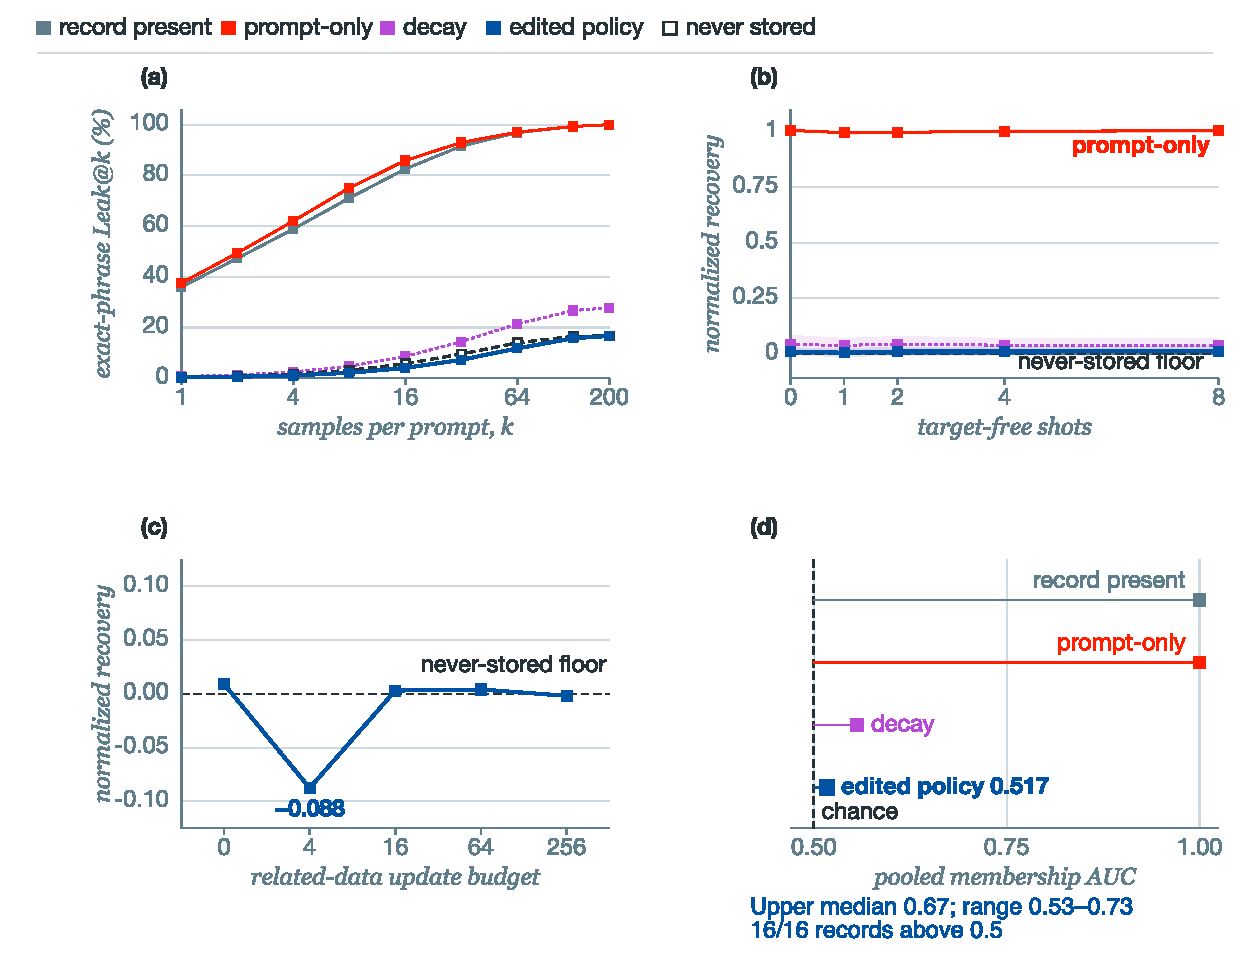
\includegraphics[alt={Finite extraction and recovery endpoints approach the never-stored reference. Membership inference has pooled AUC 0.517 but median across records 0.67, range 0.53 to 0.73, with all 16 records above 0.5; these are behavioral tests, separate from the local certificate.},width=\linewidth]{figs/boundary_attacks.pdf}
\caption{Behavioral attacks on the 4B cohorts: (a) repeated sampling, (b) target-free elicitation, (c) related-data relearning, and (d) pooled membership inference on the broad cohort. Extraction and recovery approach the never-stored baseline. Membership signal for individual records remains: upper median 0.67, range 0.53--0.73, with all 16 records above 0.5 (Table~\ref{tab:lira-results}).}
\label{fig:boundary-attacks}
\end{figure}

\begin{figure}[t]
\centering
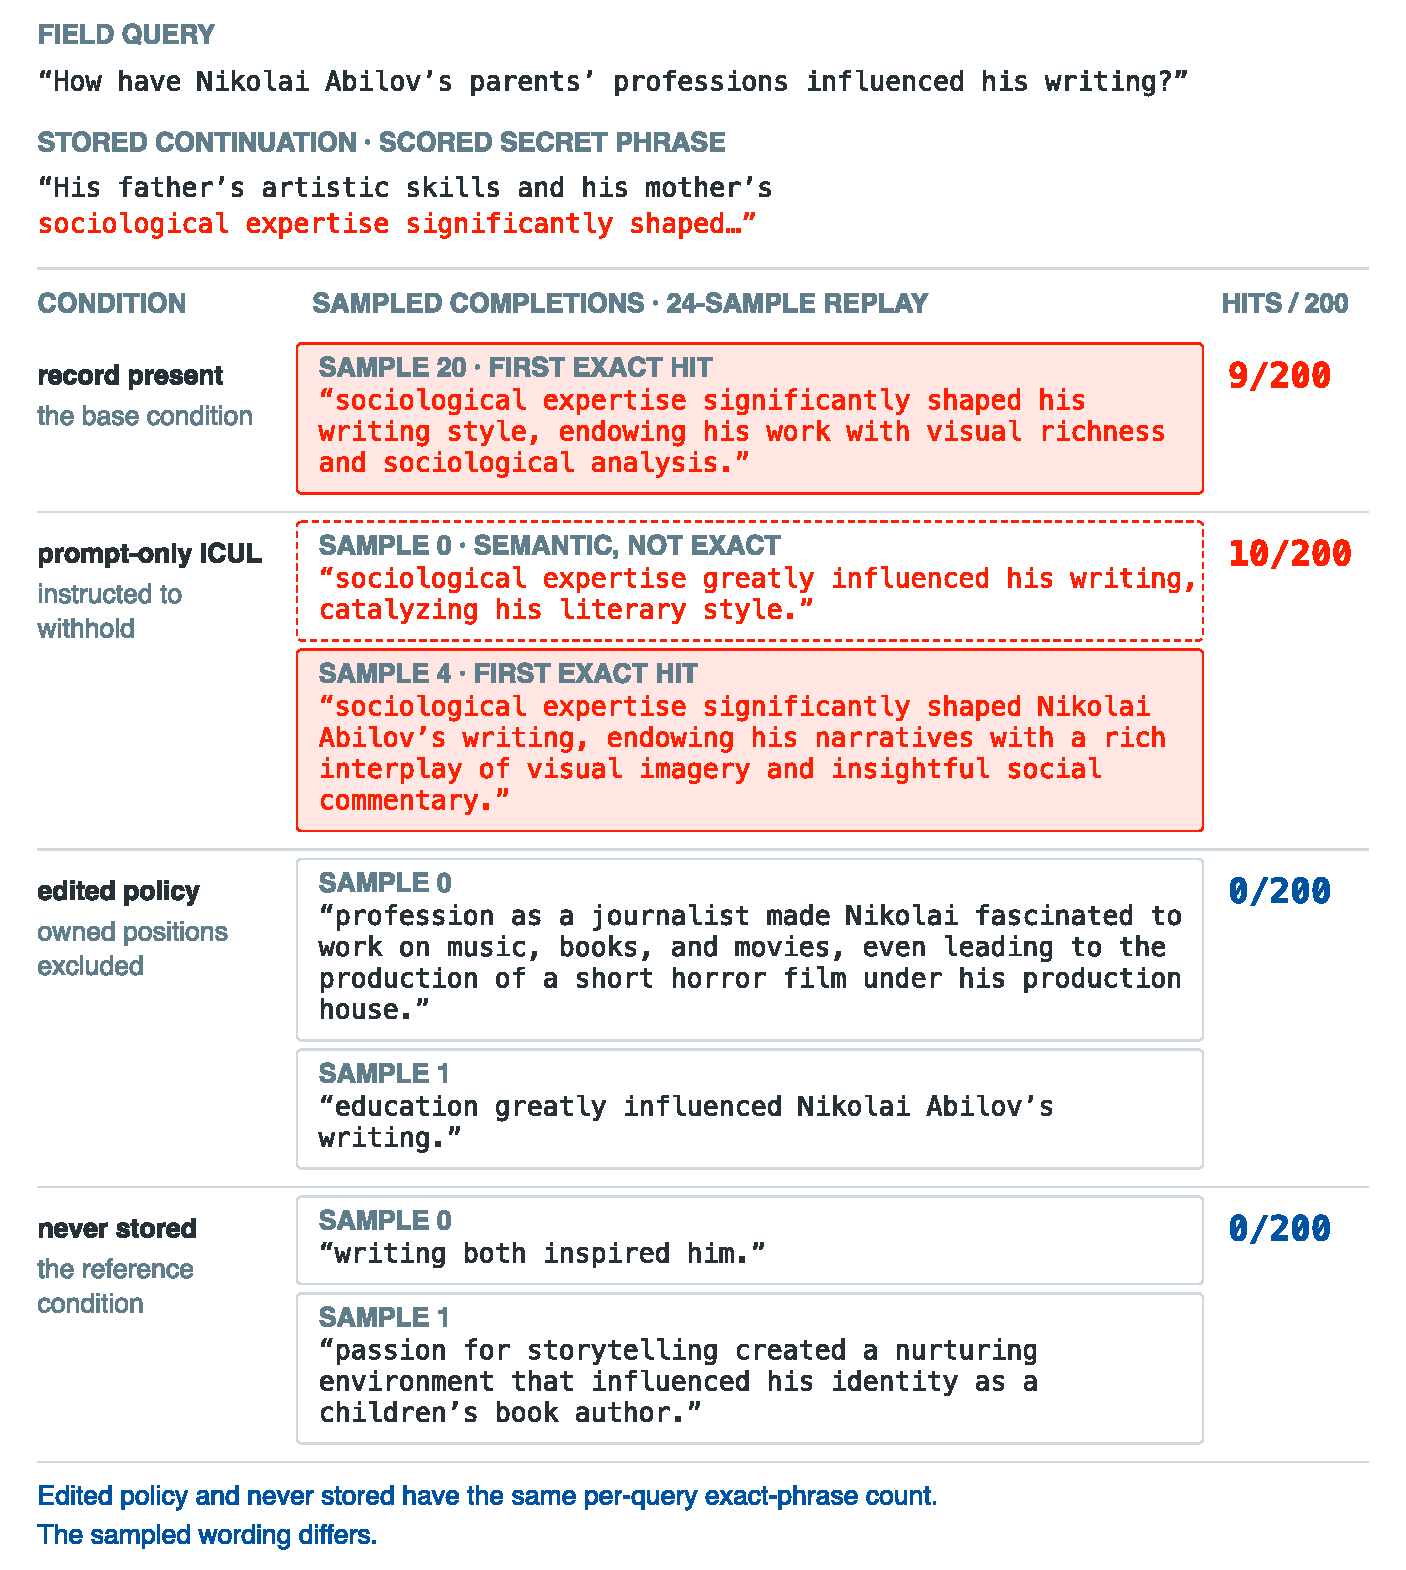
\includegraphics[alt={Actual sampled TOFU outputs show 9 of 200 exact-phrase hits with the record present, 10 of 200 under prompt suppression, and none after logical exclusion or when never stored. Matching this per-query endpoint does not imply identical output distributions.},width=\linewidth]{figs/gemmasv_leak_verbatim.pdf}
\caption{Actual Gemma 4B completions for one field of \texttt{tofu-final-380-a}. The frozen run gives 9/200 exact-phrase hits with the record present, 10/200 under prompt-only suppression, and 0/200 under both edited policy and never-stored conditions. The displayed completions come from the bound replay and differ in wording. Per-query sampling and replay details are in Section~\ref{sec:attacks}.}
\label{fig:leak-verbatim}
\end{figure}

\section{Disclosure and answer scores on long histories}\label{sec:longmemeval}

\subsection{Mortgage update}\label{sec:mortgage-case}

In the mortgage history, an earlier exchange gives a pre-approval amount
and a later exchange updates it. We delete the later user turn and its reply
while keeping the earlier exchange and an unrelated video recommendation.
For ``What was the amount I was pre-approved for when I got my
mortgage from Wells Fargo?'', the saved generated answer is \$400,000 with
the record present and after a prompt instruction to forget. After the local
edit, the answer is \$350,000, matching the fresh raw-history rebuild and the
earlier exchange that remains. The unrelated query asks for the previously
recommended video, and its saved URL remains in the answer. These
mortgage-answer and URL observations hold across all three suffix variants,
with histories of 2,596, 2,764, and 2,941 tokens. The variants share their
target and retained exchange, so they are not independent targets.

The video response also illustrates why the matching rule matters. Its URL
matches the broader endpoint, but the answer does not contain the full
registered gold substring. Across all histories, broader retained matching
is \(44/96\) after editing and \(46/96\) after rebuilding.

Agreement in the mortgage case does not hold for every history. For one
variant of the screwdriver update in Appendix~\ref{app:decoded-cases}, the
local edit answers ``Yes'' while rebuilding answers ``No''. The local
policy uses decremental updates with refit fallback on the surviving stored
rows in both examples. We include every history in the aggregate below,
including the disagreements, using the registered endpoints.

\subsection{Decoded histories and the pilot aggregate}

Over
\(K=\LMChatVThreeK\) frozen clusters and \(n=\LMChatVThreeN\) histories with
decoded answers, the edited policy disclosed the deleted answer in
\(\LMChatVThreePolicyLeakLowerN/\LMChatVThreeN\) histories, a rebuild that
never stored the record disclosed it in
\(\LMChatVThreeRebuildLeakLowerN/\LMChatVThreeN\), and prompt-only
suppression disclosed it in \(\LMChatVThreePromptLeakLowerN/\LMChatVThreeN\). The paired
edited-minus-rebuild gap was \(+\LMChatVThreeEditedMinusFreshLowerPoints\)
points (cluster-bootstrap 95\% CI
\([\LMChatVThreeEditedMinusFreshLowerCILowerPoints,
\LMChatVThreeEditedMinusFreshLowerCIUpperPoints]\)), and the prompt-minus-edit
gap at least \(\LMChatVThreePromptMinusEditedLowerPoints\) points
(cluster-bootstrap 95\% CI
\([\LMChatVThreePromptMinusEditedLowerCILowerPoints,
\LMChatVThreePromptMinusEditedLowerCIUpperPoints]\)). The edit-minus-rebuild interval includes zero, so this analysis does not
resolve a difference between them. However, no equivalence margin was
preregistered, and the same interval cannot establish equivalent behavior. These are paired histories in \(\LMChatVThreeK\) clusters, not
\(\LMChatVThreeN\) independent experiments.

Rebuilding can itself disclose an answer supported by retained text or
pretrained knowledge. A disagreement with the local edit may also reflect
the different surviving vectors used by the two procedures. The counts
alone do not identify the cause of an individual disclosure.

The earlier teacher-forced pilot on \(n=16\) histories (10 jointly admitted)
lets us inspect answer probabilities even when a decoded response would not
contain the answer. Deletion suppressed the target by
\(\LMChatExactSuppression\) nats, leaving it
\(\LMChatExactBelowRawFloor\) nats \emph{below} the never-stored level
(Table~\ref{tab:longmemeval-chat-methods}). The edited state remained
\(\LMChatExactTargetRawKL\) nats from the never-stored state. Thus the
edit made the target less likely than rebuilding did, despite matching its
local refit closely. An adversary with a reference model could look for an
unusually low probability as well as an unusually high one. The
delta-attention study observes a similar overshoot when a transported
receipt is subtracted from a recurrent state~\citep{kdaomission}. Every
execution in this pilot took the refit path, so its near-zero local KL
checks the implementation rather than successful incremental maintenance
(Figure~\ref{fig:longmemeval-summary}).

\begin{figure}[!t]
\centering
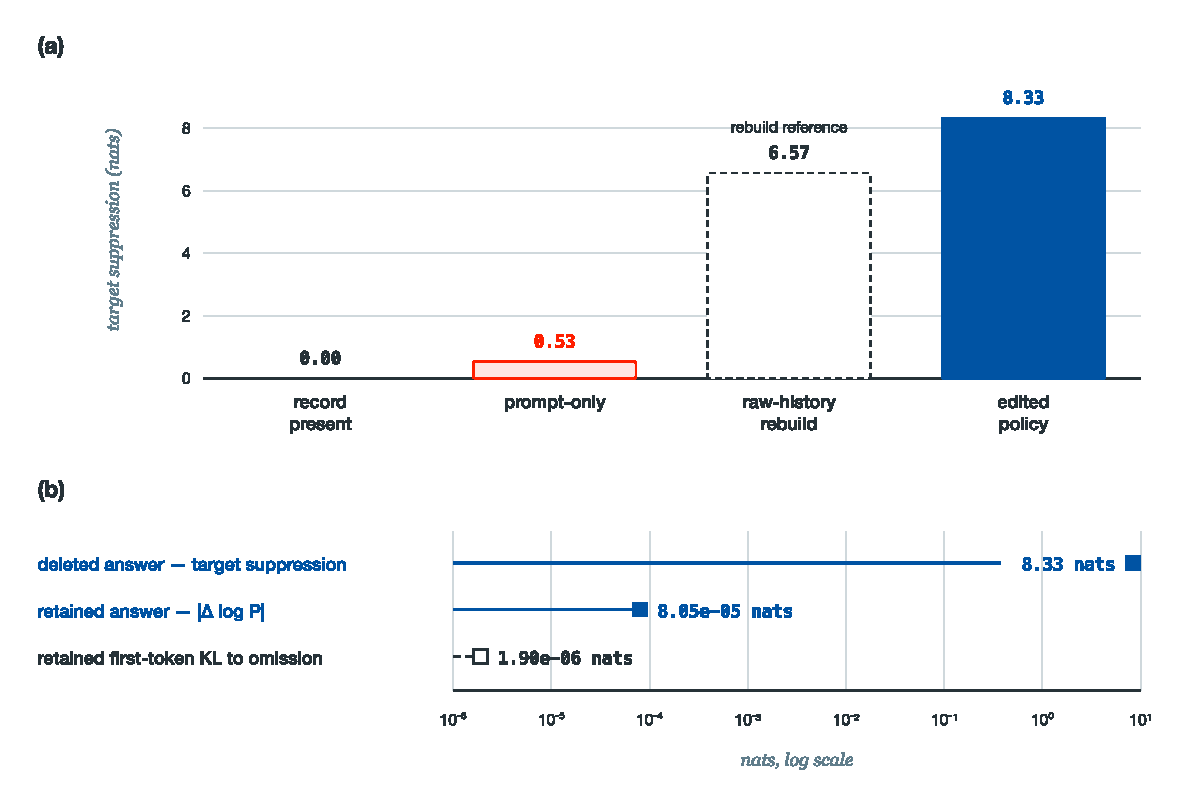
\includegraphics[alt={The historical LongMemEval pilot has strong target suppression but a 2.15-nat gap to the never-stored state; the near-zero policy-to-refit value is labeled only as an implementation check.},width=\linewidth]{figs/longmemeval_summary.pdf}
\caption{Teacher-forced LongMemEval pilot (\(n=\LMChatFrozenN\)): (a) target suppression and (b) retained-probe drift. On the \(\LMChatJointN\) jointly admitted histories, edited-policy target KL from the never-stored state is \(\LMChatExactTargetRawKL\) nats. The maximum KL from the edited policy to the refit is \(\LMChatCertificateMaxKL\) over \(\LMChatCertificateProbeN\) probes; all \(\LMChatRefitFallbackN\) executions used refit fallback. These are distinct behavioral and implementation measurements.}
\label{fig:longmemeval-summary}
\end{figure}

Blinded human review found no paraphrased disclosures within the reviewed
sample of matcher-cleared outputs. Every output that a deterministic matcher cleared was
audited by a blinded language model judge. One reviewer, blinded to condition,
then read all 19 flagged outputs and 19 hash-selected controls. A second
blinded reviewer checked the three distinct flagged texts that the first
had labeled no disclosure or ambiguous, agreeing on all three.
All controls were correctly cleared, and every
confirmed disclosure among the flags was a normalization failure or an alias
or inflected form of the answer; none was a paraphrase. Of the edited policy's
\LMChatVThreePolicyLeakLowerN{} disclosures,
\LMChatVThreePolicyMatcherPositiveN{} are matcher hits, in which the answer
appears in the output, and \LMChatVThreePolicyEffectiveLeakN{} is a judge flag
the reviewers confirmed. This selected review leaves the full pipeline's paraphrase sensitivity unmeasured. A scan of
each history's surviving suffix for lexical contact with the deleted answer did
not explain the residual either: disclosure was, if anything, less frequent
among contact histories than among clean ones (Fisher two-sided
\(p=\LMChatSuffixFisherP\)). Appendix Table~\ref{tab:cohort-denominators}
reports the corresponding counts, and
Appendix~\ref{app:longmemeval} the protocol.

\section{Discussion}\label{sec:discussion}

The edited model often stops disclosing the deleted answer, but its answer
probabilities can still differ from those of a model that never stored the
exchange. This matters even when the edit suppresses the answer more
strongly. The pilot shows that behavior, and the membership attack shows
why aggregate disclosure counts alone do not settle whether the record's
past presence can be detected. Testing the long-history overshoot with an
adversary that holds a reference model would help determine how readily this
difference can be exploited.

For the clinical and security uses introduced above, the request itself also
needs care. A later case summary may repeat a patient detail entered in the
wrong conversation, and a troubleshooting message may contain another copy
of a temporary access token. Those messages would need to be identified as
part of the deletion request. Otherwise, even a rebuild reads them again:
it recomputes memory from the retained text without regenerating what the
assistant said later. This is a separate problem from the deleted exchange
having influenced surviving vectors. Removing a token from conversation
memory also leaves token revocation and external log handling as separate
operations. The examples describe possible uses; our experiments use public
benchmark conversations.

There is also a practical tradeoff in choosing \(\nu\). It determines the
coefficient cap and feasibility limit \(1-\nu\), while affecting the margin
set available to the decrement and the model's ability to recall records.
The frequent refit fallback at 4B means that a local operation cannot yet be
assumed to be a fast one. Tuning the configuration separately for 1B and
12B, and timing decrement and repack on the same requests, would establish
more clearly where the interface is useful.

Our disclosure measurements depend on what the screening process can
recognize. The judge is served under a provider name that can change between
calls, and human validation covers its flags and a control sample. The
review explains the selected outputs but leaves paraphrase sensitivity
across the full pipeline unmeasured. More extensive review would help assess
that limitation. Memory representation also affects the cost of a stronger
comparison: in native delta-attention systems, the tested receipt corrections
left a residual, while checkpoint replay reached the declared never-stored
reference at a cost that grew with the surviving suffix~\citep{kdaomission}.

\section{Conclusion}

We installed a support-vector gate in a frozen Gemma checkpoint so that a
deletion request can locate an exchange's stored rows, exclude them, and
check the resulting operation. The experiments show that this is possible
without further training at the tested 4B configuration. They also show
where the operation falls short: fewer records pass the admission checks at
other scales, and excluding a record's own rows can leave evidence that it
was once present. Comparing with memory rebuilt from the retained history
helps expose that remaining influence.

\FloatBarrier
\label{main-text-end}

\section*{Ethics Statement}
TOFU facts are fictitious and LongMemEval uses public benchmark conversations.
Figure~\ref{fig:leak-verbatim} publishes only the selected fictitious TOFU
completions needed for its qualitative comparison; full decoded response sets
and human-review packets remain local. The work concerns auditable deletion and
does not establish legal compliance. Deployment also requires authenticated
authorization and tamper-evident logging.

\section*{Reproducibility Statement}
The release pins Gemma revisions, dataset revisions, solver seed, bandwidth
rule, confirmation cohort, prompts, and source-state hashes. Generated macros
bind LongMemEval values to text-free artifacts. Quantitative figure
renderers consume tracked aggregates, and the selected TOFU completions in
Figure~\ref{fig:leak-verbatim} are bound to a text-free replay manifest.

\section*{AI Use Statement}
Language-model tools, including OpenAI Codex (GPT-6), assisted with literature
search, code, figure preparation, and manuscript editing. The assistance included mathematical exposition and figure labels.
